\chapter{評価}
\label{evaluation}

本章では第4章の\ref{implementation}で設定した3つの実験の結果及び考察を行う。
\section{実験1 既存の活性化関数との比較実験}
\ref{exp1}で示した比較実験の結果を記述する。

\subsection{irisでの比較実験}
\label{ev:iris}

\subsubsection{設定1}


\begin{figure}[hbtp]
    \begin{center}
        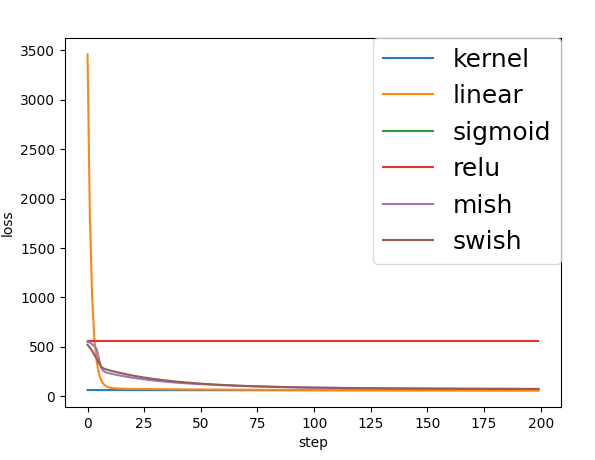
\includegraphics[width=10cm]{asset/boston_0000001_SGDkaiming_normal__non_200.png}
            \caption{Lossの比較データ}
            \label{boston}
    \end{center}
\end{figure}


\begin{table}[htbp]
    \begin{center}
        \caption{設定1の結果まとめ}
        \vspace{5mm} 
        \begin{tabular}{l*{2}{c}r}
            活性化関数              & loss \\
            \hline
            K-AF            & 0.0 \\
            Sigmoid            & -22.0 \\
            Linear            & 0.0 \\
            ReLU        & -22.0 \\
            Swish           & 0.0 \\
            Mish           & -1.0 \\
    
        \end{tabular}
    \end{center}
\end{table}

\subsubsection{設定2}

\begin{figure}[hbtp]
    \begin{center}
        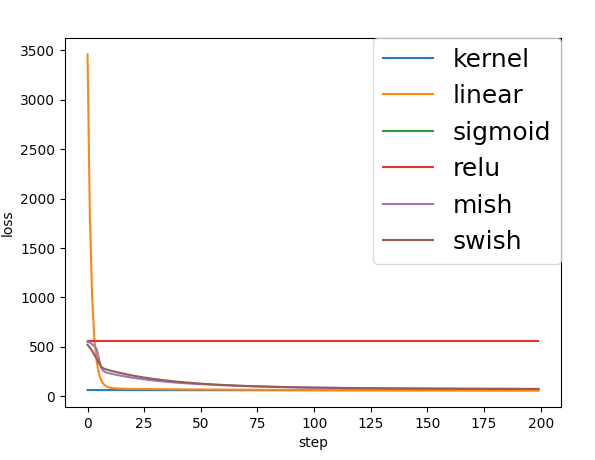
\includegraphics[width=10cm]{asset/boston_0000001_SGDkaiming_normal__non_200.png}
            \caption{Lossの比較データ}
            \label{boston}
    \end{center}
\end{figure}


\begin{table}[htbp]
    \begin{center}
        \caption{設定1の結果まとめ}
        \vspace{5mm} 
        \begin{tabular}{l*{2}{c}r}
            活性化関数              & loss \\
            \hline
            K-AF            & 0.0 \\
            Sigmoid            & -22.0 \\
            Linear            & 0.0 \\
            ReLU        & -22.0 \\
            Swish           & 0.0 \\
            Mish           & -1.0 \\
    
        \end{tabular}
    \end{center}
\end{table}


\subsubsection{irisまとめ}

irisでは十分な性能を出すことができた。


\subsection{digitsでの比較実験}
\label{ev:digitsでの比較実験}

\subsection{wineでの実験と設定}
\label{ev:wineでの実験と設定}

\subsection{bostonでの比較実験}
\label{ev:bostonでの比較実験}

\subsection{breast\_cancerでの比較実験}
\label{ev:breastcancer}

\section{実験2 K-AFの関数形状の調査}
\ref{exp1}で示した比較実験の結果を記述する。


\begin{figure}[hbtp]
    \begin{center}
        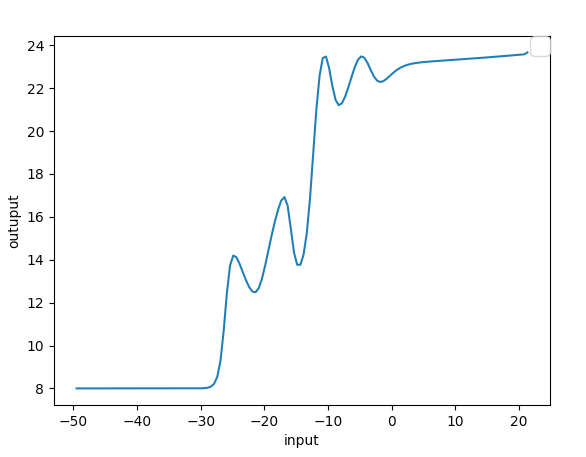
\includegraphics[width=10cm]{asset/boston_0000001_SGDkaiming_normal__non_200_function_2.png}
            \caption{活性化関数の形}
            \label{boston}
    \end{center}
\end{figure}


\section{実験3 K-AFの性能が上がる条件探査}
\ref{exp1}で示した比較実験の結果を記述する。

\section{まとめ}

K-AFの精度、勾配消失の有無、実用性の観点から先行研究との比較を行った. 実験結果を
踏まえ, 第 6 章で考察を行う.


%%% Local Variables:
%%% mode: japanese-latex
%%% TeX-master: "./thesis"
%%% End:
